\documentclass[border=3pt,tikz]{standalone}
\usepackage{amsmath}
\usetikzlibrary {3d} 
\usetikzlibrary {arrows}
\usetikzlibrary{shapes.geometric}
\begin{document}
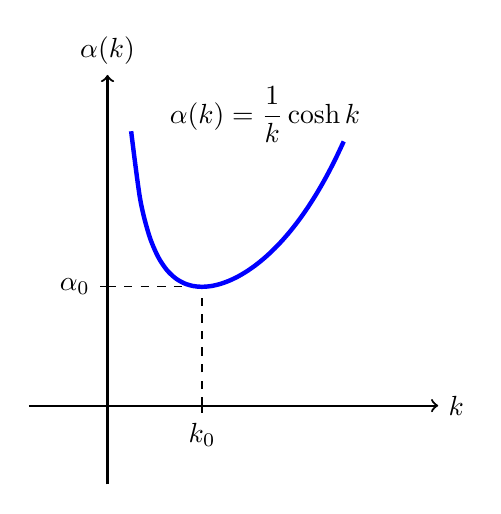
\begin{tikzpicture}[=>stealth, scale=1]
  \draw[thick, ->] (-1,0) -- (4.2,0) node[right] {$k$};
  \draw[thick, ->] (0,-1) -- (0,4.2) node[above] {$\alpha(k)$};
  \draw[, -] (1.2, 0.1) -- (1.2 ,- 0.1) node[below] {$k_0$};
  \draw[-] (0.1, 1.51)-- (-0.1, 1.51) node[left] {$\alpha_0$};
  \draw[dashed] (0.0, 1.51) -- (1.2, 1.51) ;
  \draw[dashed] (1.2, 0) -- (1.2, 1.51) ;
  \draw[scale=1.0,domain=0.3:3,smooth,variable=\x,blue, ultra thick] plot ({\x},{1./\x * cosh (\x)});
  \node[] at (2, 3.7) {$\alpha (k) = \dfrac{1}{k} \cosh k$};
  %\draw[scale=0.5,domain=-3:3,smooth,variable=\y,red]  plot ({\y*\y},{\y});
\end{tikzpicture}
\end{document}